\section{Speech in communication}

This section will analyse the human speech intelligibility with respect to the frequency range for the human through communication channel e.g. air, bone or electronic systems. The intelligibility of a speech depends on the sound quality, noise and the frequency range of the voice. This section will focus on the frequency of the the voice, to determined the necessary frequency range in electronic systems for communication. 

The intelligibility of the voice is an important factor in communication and are therefore a factor in the frequency range of the human voice. The fact that the fundamental frequency for the voice is in the low frequency area does not necessary mean that all high frequency above that fundamental frequency area can be filtered away. The overtone of the voice might affect the intelligibility of speech. Therefore the intelligibility of speech is the focus area of this reachurch of the voice frequency range. 

One on the most important acoustics factor in the human speech is the glottal oscillation, which is fundamental frequency of the voice. The fundamental frequency is person dependent but the mean differs from male and female and the type of communication e.g. song speech or jelling. For male the mean fundamental frequency for conversational speech is \SI{120}{\hertz} and for female is is \SI{200}{\hertz}. The fact that the fundamental frequency is that low does not mean that those frequency are important in the frequency range for the human conversational speech output of the mouth. The throat speaking system contain a transfer function from the the glottal oscillation to the output of a mouth \citep{pulkki2015}. The following \autoref{fig:speech_system} shows the path way for the air from the glottal to the lips.


 \begin{figure}[H]
	\centering
		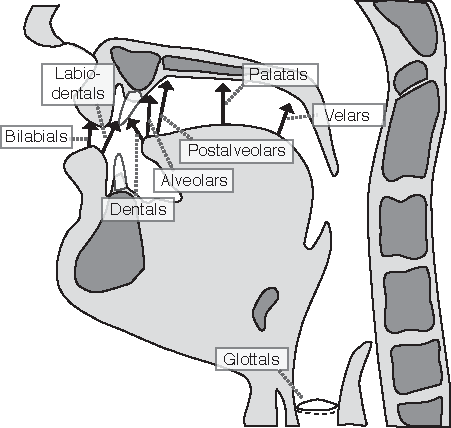
\includegraphics[width=1\textwidth]{glottal}
		\caption{The figure shows the path way from the glottal to the lips \citep{pulkki2015}}
		\label{fig:speech_system}
\end{figure}

The transfer function is human depending and more specific throat depending. The mean length for the throat from generation of the glottal oscillation to the lips is \SI{17}{\centi\meter} for male and \SI{14}{\centi\meter} for female. glottal oscillation is mixed with unvoiced airflow in the throat which make turbulence in the transfer for voice. This generate e.g. noise and explosive transient-like sound in the voice output \citep{pulkki2015}. The following \autoref{fig:speech_transfer_system} shows a signal block diagram for the speech transfer function.

 \begin{figure}[H]
	\centering
		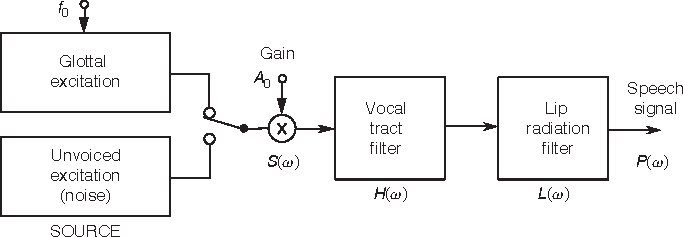
\includegraphics[width=1\textwidth]{speech_transfer}
		\caption{The figure shows a block diagram for the speech transfer function \citep{pulkki2015}}
		\label{fig:speech_transfer_system}
\end{figure}


In fact with the speech transfer function the frequency range can start below \SI{100}{\hertz} and go upon several \si{\kilo\hertz}. In language depending speech there is some low frequency fundamental component generating by the tongue there goes down to \SI{20}{\hertz}. The tongue is generating it by trilling e.g. "r'' in Spanish. The highest frequency component is generated by singing and goes up to \SI{7}{\kilo\hertz} \citep{pulkki2015}.

At this point all frequency above  \SI{7}{\kilo\hertz} do not affect the intelligibility of the voice, since the voice do not generate frequency above. The range from \SI{20}{\hertz} to \SI{7}{\kilo\hertz} is then the outer limit but the frequency area might not be that wide when it is the intelligibility that is of important. Filtering away some of the frequency might not affect the speech intelligibility. 

For fully understand what there is needed for good speech intelligibility, the speech intelligibility meaning has to be fully understood. The speech intelligibility is as measure of how much of a message has been extracted from the recognized phonemes. Phonemes is the smallest unit of speech \citep{arl_us_army}. This measure indicate how good words and sentences can be understood in a listening event. The speech intelligibility can be limited to \SI{1}{\kilo\hertz} to \SI{6}{\kilo\hertz} where it is expressed in percentage of received speech. The power spectrum of the speech which is explained earlier in this section which goes from  \SI{100}{\hertz} up to \SI{7}{\kilo\hertz} is not correlated to the speech intelligibility, which mean that not all frequency of the voice affect the speech intelligibility. Most of the speech power is distributed near the fundamental frequency of the voice, but for speech intelligibility measure it is below \SI{5}{\percent}. Therefore when hearing speech, the frequency of the voice might not be observed as it low fundamental frequency but much higher. in fact \SI{60}{\percent} of the speech intelligibility lays in only \SI{5}{\percent} of the speech power spectrum \citep{arl_us_army}. The spectral centroid of the speech intelligibility frequency are various from language but not fare away from each other. For the English language the centroid is a \SI{1.5}{\kilo\hertz} \citep{arl_us_army}. The following \autoref{fig:speech_intelligibility} shows the power and intelligibility in octave. 


 \begin{figure}[H]
	\centering
		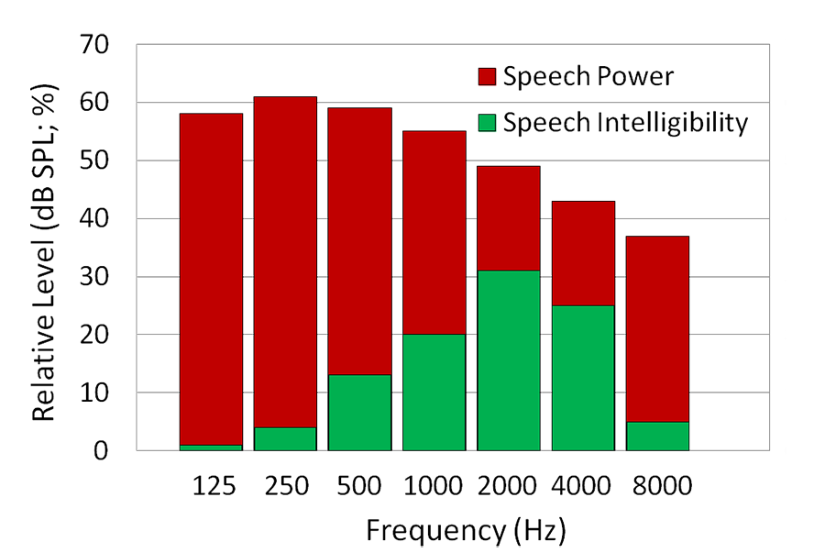
\includegraphics[width=1\textwidth]{speech_intelligibility}
		\caption{The figure shows the power and intelligibility in octave  \citep{arl_us_army}}
		\label{fig:speech_intelligibility}
\end{figure}

As it can be seen at \autoref{fig:speech_intelligibility} the frequency range can be further limited to the range \SI{355}{\hertz} up to \SI{5.68}{\kilo\hertz} because of the outer low frequency limit of \SI{500}{\hertz} and the upper outer high frequency limit for \SI{4} for octave band. 

In word the vowels and consonants are not equally distributed for speech intelligibility, in fact they are fare away from each other. For speech intelligibility the consonant is the dominant part, and the reason shall be founded in the difference between speech power and speech intelligibility \autoref{fig:speech_intelligibility}. The vowel is actually the letters with the highest power and in the low frequency region, where the consonant is of less power but in higher frequency. With this in mind the consonants is the important for speech intelligibility where vowel do not matter.




